\documentclass[a4paper, 12 pt, italian]{report}

\usepackage[T1]{fontenc}
\usepackage[utf8]{inputenc}
\usepackage[italian]{babel}

\usepackage{graphicx}

\setcounter{tocdepth}{2}
\begin{document}

\title{JavaRMI}

\author{Frasca Luigi \and Gargano Riccardo}
\date{12 Dicembre 2014}


\maketitle

\begin{abstract}
Dopo aver studiato il vasto programma del corso di Reti di Calcolatori abbiamo incentrato il nostro progetto su una particolare tecnologia, la Remote Method Invocation(RMI).\\
Abbiamo progettato e implementato un'applicazione di messaggistica basata su RMI.\\
L'applicazione \'e stata realizzata in Java che offre una tecnologia specifica, la Java Remote Method Protocol, per la ricerca e il riferimento a oggetti remoti.\\
Con questa stesura vogliamo spiegare gli argomenti analizzati e trattati che ci hanno permesso di riuscire nel nostro scopo.

\end{abstract}


\tableofcontents


\chapter{Introduzione}
\section{Socket}

I Sistemi Distribuiti, per loro natura, prevedono che computazioni differenti possano essere eseguite su Virtual Machine differenti, possibilmente su host differenti, comunicanti tra loro.\\
Al fine di consentire la programmazione di sistemi distribuiti (in rete) il linguaggio Java supporta la nozione di socket, un meccanismo flessibile e potente per la programmazione di sistemi distribuiti.\\
I socket sono un meccanismo di basso livello e, come tutti i linguaggi a basso livello, presentano una serie di difficolt\'a per il programmatore.
Con i socket le difficolt\'a maggiori derivano dall'eterogeneit\'a delle entit\'a in rete. Occorre definire un "protocollo" per l'invio delle richieste di servizio e delle risposte, con relativa codifica e decodifica dei parametri in sequenze di byte.

\section{RPC}
Un'alternativa ai sockets \'e rappresentato da una tecnologia di pi\'u alto livello, comunemente chiamata RPC (Remote Procedure Call), in cui l'interfaccia di comunicazione \'e rappresentata dall'invocazione (remota) di procedura.
La tecnologia RPC consente di invocare procedure che appartengano ad applicazioni remote, in maniera del tutto trasparente all'utente.\\
Pi\'u precisamente il client invoca una procedura del server remoto, il quale si occupa di eseguire la procedura (con i parametri passati dal client) e di ritornare a quest'ultimo il risultato dell'esecuzione.\\
La connessione remota \'e trasparente al client che ha l'illusione di invocare una procedura locale.\\
Grazie alla RPC, il programmatore non deve pi\'u preoccuparsi di sviluppare dei protocolli che si occupino del trasferimento dei dati, della verifica, e della codifica/decodifica. Queste operazioni sono interamente gestite dalla RPC.
La tecnologia RPC presenta comunque dei limiti:
\begin{itemize}

\item parametri e risultati devono avere tipi primitivi.

\item la programmazione \'e essenzialmente procedurale.

\item non vi \'e programmazione ad oggetti e quindi mancano i concetti di ereditariet\'a, incapsulamento, polimorfismo, etc..

\end{itemize}


\section{Middleware}

A partire dagli inizi degli anni '90 sono state proposte delle tecnologie, dette Middleware, per superare i limiti di RPC:
\begin{itemize}

\item CORBA: supporta applicazioni scritte in linguaggi differenti su piattaforme differenti.

\item Java RMI: supporta applicazioni Java su una piattaforma Java, le applicazioni possono essere distribuite su differenti Java Virtual Machine.

\item DCOM: supporta applicazioni scritte in linguaggi differenti, ma su piattaforme Win32. Esistono delle implementazioni per sistemi Unix.

\item .NET remoting: supporta applicazioni scritte in linguaggi differenti, su piattaforma Windows.


\end{itemize}

\chapter{Java Remote Method Invocation}

\section{Cos\'e Java RMI}
Java RMI \'e una tecnologia che consente a processi distribuiti di comunicare attraverso la rete.\\

L'idea alla base di tutta la programmazione distribuita \'e semplice
\begin{itemize}
\item Un client esegue una determinata richiesta. Tale richiesta viaggia lungo la rete verso un determinato server destinatario

\item Il server processa la richiesta e manda indietro la risposta al client per essere analizzata

\item Con i socket per\'o dobbiamo gestire personalmente il formato dei messaggi e la gestione della connessione

\end{itemize}
Java RMI permette l'accesso ad oggetti remoti (cio\'e su altri nodi della rete Internet) come se fossero oggetti locali, senza doversi preoccupare della realizzazione della connessione, degli stream di input e output, etc..\\
Quindi possiamo definire Java RMI un insieme di strumenti, politiche e meccanismi che permettono l'invocazione remota di metodi su oggetti che risiedono su diverse Java Virtual Machine.\\
\\
Vantaggi nell'utilizzare Java RMI:

\begin{itemize}

\item \'E un linguaggio ad oggetti, i concetti di riutilizzabilit\'a (ereditariet\'a), protezione dell'informazione (incapsulamento), ed accesso dinamico (polimorfismo) sono gi\'a definiti.

\item Consente il passaggio di referenze ad oggetti remoti.

\item Supporta un Java Security Manager per controllare che le applicazioni distribuite abbiano i diritti necessari per essere eseguite.

\item Supporta un meccanismo di Distributed Garbage Collection (DGB) per disallocare quegli oggetti remoti per cui non esistano pi\'u referenze attive.

\end{itemize}

\section{Stub \& Skeleton}
Questa architettura adotta il proxy pattern, i due proxy (\textbf{stub} dalla parte client e \textbf{skeleton} dalla parte server) nascondono al livello applicativo la natura distribuita dell'applicazione.\\

\begin{itemize}

\item Il server istanzia degli oggetti remoti e li rende visibili.

\item Gli oggetti remoti implementano una determinata interfaccia remota che dichiara i metodi accessibili dall'esterno.

\item I client ottengono dei riferimenti agli oggetti remoti, Stub, tramite i quali possono invocare i metodi remoti dichiarati.

\end{itemize}
Quindi, un client non accede a un server remoto direttamente, ma attraverso lo stub, il quale va in esecuzione sulla macchina del client ed agisce da rappresentante locale (proxy) al server remoto.\\
Un oggetto stub traduce automaticamente ogni invocazione al server remoto in termini di comunicazione di rete, con relativo passaggio di parametri ed eventuale codifica/decodifica (marshalling / unmarshalling).\\
Definiamo allora lo stub come una referenza al server remoto. Referenza di cui il client deve necessariamente venire in possesso se vuole invocare i metodi del server remoto.\\
Lo stato di un oggetto stub contiene essenzialmente tre informazioni: 
\begin{itemize}

\item l'IP dell'host su cui gira il server.
\item la porta su cui \'e in esecuzione il server.
\item un identificativo RMI associato al server remoto.
\end{itemize}
Esiste, invece, sul server un proxy del client lo skeleton. Il suo compito \'e quello di ricevere presso l'host del server le richieste da parte dello stub decodificarle, inoltrarle al server, codificare i risultati ed inviarli allo stub affinch\'e li passi al client.
\newpage

\section{Architettura RMI}
Esiste un programma speciale che agisce da "Naming Service", in Java \'e il RMI Registry.


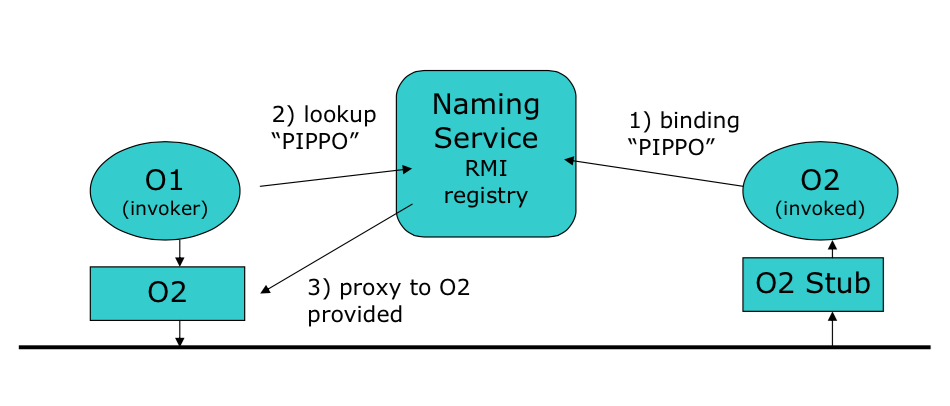
\includegraphics[]{schema1}




\begin{itemize}

\item registra i nomi e i riferimenti degli oggetti i cui metodi possono essere invocati da remoto (O2 nella figura).

\item tali oggetti devono registrarsi, fare il "bind" presso il naming service, con un nome pubblico("PIPPO" nella figura).

\item altri oggetti possono richiedere, fare il "lookup" di oggetti registrati chiedendo, a partire dal nome pubblico, un riferimento all'oggetto

\end{itemize}
Quando il Naming Service riceve una richiesta di lookup, corrispondente a un oggetto che lui conosce (nella figura, il Naming Service sa che l'oggetto di nome pubblico "PIPPO" corrisponde all'oggetto O2, allora:


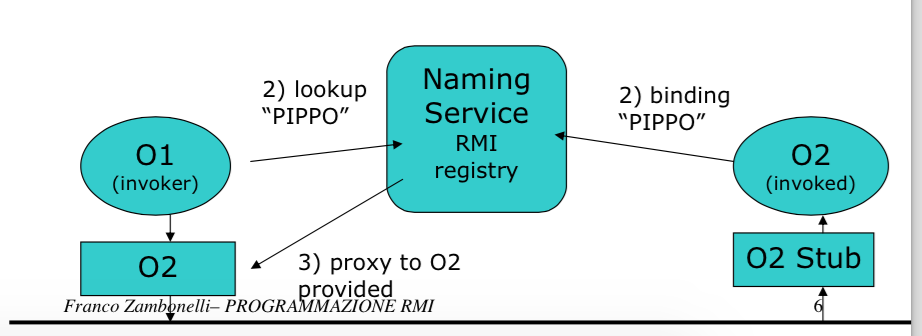
\includegraphics[]{schema2}

\begin{itemize}

\item viene generato un oggetto "virtuale", lo "skeleton", che viene inviato presso il nodo di colui che aveva richiesto il lookup (O1 in figura).

\item dal punto di vista di O1, esso percepisce il proxy di O2 come un normale riferimento a un oggetto O2 locale.

\end{itemize}

In verit\'a, quando O1 chiede un servizio a O2, lo chiede al suo proxy che:
\begin{itemize}

\item senza che O1 se ne accorga, stabilisce una connessione Socket TCP con il nodo dove c'\'e O2 vero.

\item in tale nodo di O2, un componente associato a O2, lo "stub" riceve la connessione e la richiesta di servizio, e provvede a invocarla lui su O2 vero.

\item quando O2 vero risponde, lo stub manda la risposta indietro al proxy, il quale poi risponde a O1 come se fosse stato realmente lui a eseguire il servizio.

\end{itemize}
\newpage

\section{Creare un'applicazione in Java RMI}

\subsection{Progettazione ed Implementazione delle componenti distribuite}

Si decide la struttura dell'applicazione e si stabilisce quali funzionalit\'a devono essere espletate da oggetti locali e quali da server remoti.\\
Vi sono sostanzialmente tre diversi moduli la cui progettazione richiede particolare cura:

\begin{itemize}

\item \textit{Definizione dell'interfaccia remota.} Un'interfaccia remota \'e una particolare interfaccia Java che denota quei metodi del server che possono essere invocati remotamente da un client. \\
Tale interfaccia remota deve essere conosciuta sia dal server che dal client. Quest'ultimo, infatti, deve conoscere il nome dei metodi remoti ed il tipo dei parametri e dei risultati che vengono passati. \\
L'interfaccia remota rappresenta quindi la modalit\'a attraverso cui un client ed un server interagiscono tra loro.\\
Un'interfaccia remota per definirsi tale deve estendere l'interfaccia 
\begin{verbatim}
java.rmi.Remote 
\end{verbatim}
Tutti i metodi che appartengono ad un'interfaccia remota devono lanciare 
\begin{verbatim}
java.rmi.RemoteException
\end{verbatim}
\item \textit{Implementazione dei server remoti.} I server remoti devono implementare una o pi\'u interfacce remote. Un server pu\'o implementare pi\'u di una interfaccia remota nel caso voglia fornire "views" differenti a client differenti.
L'implementazione di un oggetto remoto deve estendere la classe 
\begin{verbatim}
java.rmi.server.RemoteObject
\end{verbatim}
o una sua sottoclasse, e deve implementare tutte le interfacce remote che intende supportare.


\item \textit{Implementazione dei client.} Clienti che interagiscono con server remoti possono essere implementati in ogni momento, anche successivamente all'implementazione del server, purch\'e facciano un uso appropriato dell'interfaccia remota per accedere il server.

\item \textit{Lancio del registro RMI.} Prima di lanciare il server remoto (e quindi l'applicazione client) \'e necessario lanciare presso il server il registro di Naming RMI. \\
In modo che il client possa recuperare le referenze ai server remoti di cui ha bisogno.
Il registro di naming pu\'o essere lanciato da linea di comando:
\begin{verbatim}
rmiregistry
\end{verbatim}
Il registro RMI presso l'host del server \'e semplicemente identificato con l'IP dell'host e la porta su cui \'e in esecuzione il registro (di default la 1099).
\item \textit{Lancio del server.} Dopo essere stato lanciato il server viene messo in ascolto su una porta (definibile dall'utente) da cui accetta richieste di invocazioni remote da parte del sistema RMI. 

\item \textit{Registrazione del server remoto sul registro RMI.} Il server remoto pu\'o essere registrato sul registro RMI, in modo che gli altri client possano ottenere la referenza remota (stub) per accedere al server.

\end{itemize}

\newpage

\subsection{Compilazioni sorgenti e generazioni stub}
La compilazione avviene in due fasi:

\begin{itemize}

\item Nella prima si utilizza il compilatore \textbf{javac} per compilare i sorgenti del server e del client. Pi\'u precisamente presso il server si compilano le interfacce remote e l'implementazione del server, mentre sulla macchina client si compilano l'interfaccia remota e l'applicazione client (l'interfaccia remota deve essere conosciuta sia dal server che dal client).\\

\item Nella seconda fase si usa il compilatore \textbf{rmic} per generare nella macchina server le classi stub e skeleton relative ai server remoti. 
\\
\textbf{NOTA} A partire dalla J2SE 5.0 tale compilazione non sarebbe pi\'u necessaria in quanto le classi stub vengono create a tempo d'esecuzione. \\
Il compilatore \textbf{rmic} va comunque usato quando si ha a che fare con clients che utilizzano versioni precedenti di Java.
\begin{verbatim}
rmic ServerRemoto
\end{verbatim}
Questo comando produce le classi
\begin{verbatim}
ServerRemoto_Stub.class e ServerRemoto_Skel.class. 
\end{verbatim}
Entrambi le classi sono necessarie per l'esecuzione dell'implementazione dell'oggetto remoto.\\
Un client in possesso di una referenza remota, ovvero un oggetto stub, per poterlo utilizzare deve accedere alla classe di appartenenza dell'oggetto stub:
\begin{verbatim}
ServerRemoto Stub.class
\end{verbatim}

\textbf{NOTA} quando un client riceve uno stub oltre a ricevere l'oggetto stub caricher\'a dinamicamente in maniera trasparente la classe dell'oggetto stub attraverso un meccanismo detto \textbf{codebase} che in Java RMI gioca un ruolo molto importante durante la trasmissione di referenze remote.

\end{itemize}

\chapter{La nostra applicazione}

\section{Login}
Per poter utilizzare la nostra applicazione \'e necessario effettuare un login con credenziali(user e password).\\Queste credenziali vengono controllate tramite la funzione:
\begin{verbatim}
boolean validate(String user, String pwd, ClientInterface client)
\end{verbatim}
che attraverso l'invocazione remota ci permette di controllare le credenziali sul server, se queste sono corrette il server registra in un \textbf{HashMap usersOn} l'username e l'interfaccia remota che servir\'a per comunicare con lo specifico client.\\
Le credenziali se sbagliate per 3 volte consecutive producono l'uscita dall'applicazione.\\
La password prima di essere inviata al server viene codificata con un Message Digest, in questo caso MD5, questo tipo di codifica prende in input una stringa di lunghezza arbitraria e ne produce in output un'altra a 128 bit.\\
L'MD5 \'e standardizzato con la RFC 1321.
\subsection{Autenticazione CAS}
Central Authentication Service (CAS) \'e un servizio per l'autenticazione Single Sign-On (SSO) di una comunit\'a Web.\\
Le applicazioni demandano il problema dell'autenticazione al server centrale CAS, senza pi\'u preoccuparsi dei vari problemi di identificazione dell'utente.\\
L'utente dovr\'a autenticarsi una sola volta, ad esempio con username e password, o con l'invio di un certificato digitale, e da quel momento in poi potr\'a utilizzare tutte le applicazioni fornite dal sistema, senza doversi autenticare nuovamente, finch\'e la sessione \'e valida.\\
Il CAS \'e composto principalmente da due componenti:
\begin{itemize}
\item Il CAS server, che gestisce l'identita' della comunita'.
\item I Service Providers, che forniscono le applicazioni che richiedono accesso autenticato.
\end{itemize}
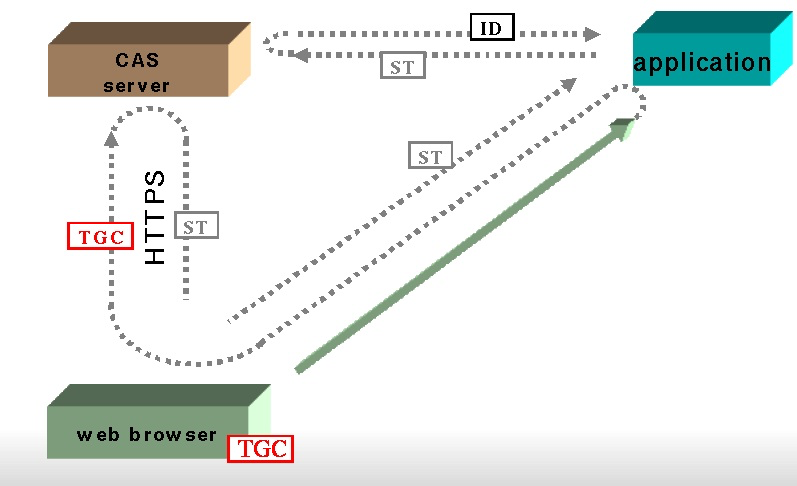
\includegraphics[height=50mm, width=100mm]{cas}\\
Gli scopi principali del server CAS sono:
\begin{itemize}
\item Facilitare l'autenticazione centralizzata SSO per pi\'u applicazioni comuni.
\item Semplificare la procedura stessa di autenticazione
\item Consentire un autenticazione sicura agli utenti, senza che questi debbano
rivelare le proprie credenziali ai servizi e agli applicativi ogni volta.
\end{itemize}
Per quel che riguarda l'autenticazione, le credenziali dell'utente viaggiano solo una volta tra il browser dell'utente ed il server su un canale protetto e crittografato in SSL. \\
Durante l'autenticazione, il server CAS cerca di salvare nel browser dell'utente uno speciale cookie privato: il Ticket Granting Cookie, TGS. Questo non contiene nessun tipo di dato confidenziale, ma contiene solamente un identificativo di sessione noto al CAS. \\
Il ticket ha comunque un tempo di vita relativamente breve, e viene cancellato definitivamente alla chiusura del browser da parte dell'utente.\\
Questo speciale ticket, serve come garanzia di avvenuta autenticazione qualora l'utente intenda accedere ad un'altra applicazione del sistema. In questo modo l'utente in tutta trasparenza non deve re-autenticarsi ogni volta che cambia il servizio applicativo richiesto.\\
Le applicazioni invece non comunicano attraverso il ticket TGT, ma attraverso
altri ticket appositi, detti Service Ticket, ST. \\
Essi non contengono informazioni personali, e possono essere utilizzati solo una volta (one time ticket). Il ST viene emesso dal server CAS verso l'utente, il quale in modo automatico lo passa al servizio applicativo. Questi lo ridirige di nuovo verso il CAS per confermare l'identit\'a dell'utente, chiudendo il ciclo di autenticazione.
\section{Interfaccia Utente}
Il login della nostra applicazione si presenta cos\'i:\\\\
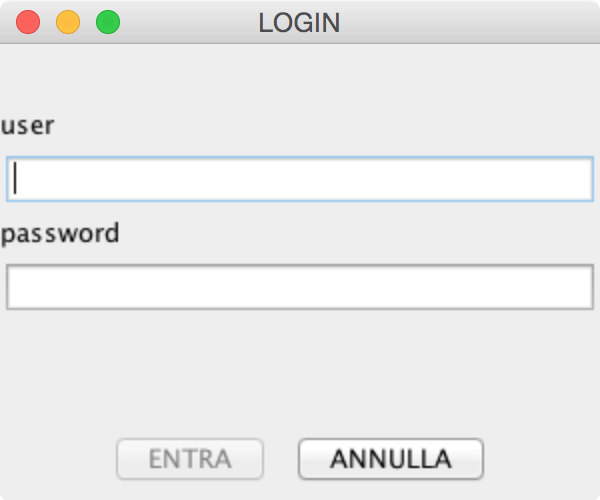
\includegraphics[height=50mm, width=80mm]{login}
\\
Dopo aver effettuato il login, visualizziamo la finestra che elenca tutti gli utenti connessi alla chat:\\\\
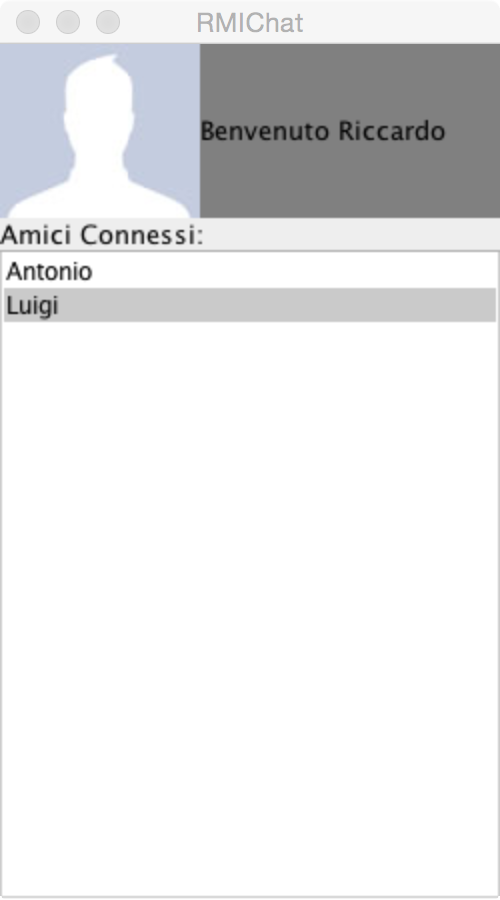
\includegraphics[height=80mm, width=50mm]{window}\\\\
In seguito \'e possibile avviare una singola conversazione con l'amico desiderato:\\\\
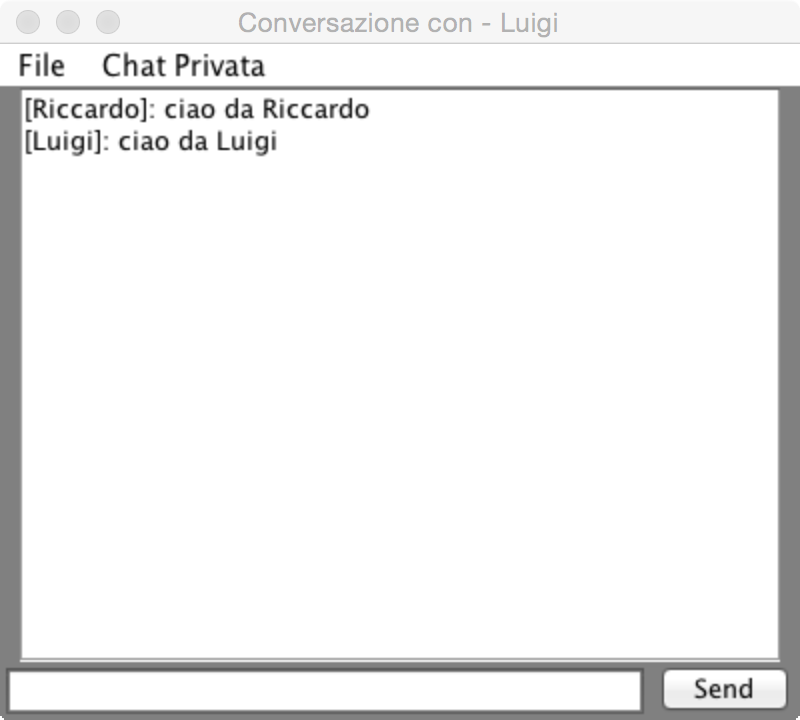
\includegraphics[height=70mm, width=70mm]{conv}\\







\section{Scambio di Messaggi}
All'interno della nostra applicazione definiamo due interaccie remote :

\begin{verbatim}
public interface ServerInterface extends Remote
public interface ClientInterface extends Remote
\end{verbatim}
Nello specifico la ServerInterface definisce il seguente metodo

\begin{verbatim}
public void sendMessageTo(int mode, String mitt, String dest, byte[] msg)
\end{verbatim}
il quale dopo aver effettuato una ricerca all'interno dell'HashMap \textbf{usersOn}, ove gli verr\'a restituita la ClientInterface di destinazione sulla quale chiamare il metodo definito in essa :
\begin{verbatim}
public void tell(int type, String user,byte[] msg)
\end{verbatim}
che permetter\'a lato client di visualizzare il messaggio su un'apposita finestra di comunicazione. Lo scambio di messaggi pu\'o avvenire in modo criptato.

\section{Crittografia}
\subsection{Introduzione}
Il crescente utilizzo di internet come mezzo per lo scambio rapido di informazioni, ha enfatizzato la necessit\'a di comunicazioni sicure, private, protette da sguardi indiscreti. \\
Sfortunatamente la rete, cos\'i come \'e stata concepita, non supporta un buon livello di sicurezza e di privacy. Le informazioni viaggianti sono trasmesse in chiaro e potrebbero essere intercettate e lette da qualsiasi individuo. \\
Pertanto  \'e stato necessario creare dei metodi che, rendano le informazioni indecifrabili in modo che solo il mittente e il destinatario possano leggerle, e ne assicurino l'integrit\'a.
\subsection{Algoritmi a chiave simmetrica}
Gli algoritmi a chiave simmetrica usano la stessa chiave per cifratura e decifratura. Entrambi gli interlocutori conoscono la chiave usata per la cifratura, detta chiave privata, e soltanto loro possono cifrare e decifrare il messaggio.\\
\begin{verbatim}
MessaggioCriptato = E(Chiave,Messaggio)
Messaggio = D(Chiave,MessaggioCriptato)
\end{verbatim}
dove E e D sono cipher noti.\\
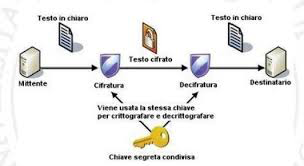
\includegraphics[height=75mm, width=150mm]{simmetrica}
\subsection{Algoritmi a chiave pubblica}
La cifratura a chiave simmetrica ha una grave debolezza nel trasferimento della chiave per renderla condivisa.\\
Diffie ed Hellmann nel 1976 proposero una tecnica nuova di crittografia, basata sull'aritmetica modulare, in cui vengono utilizzate due chiavi Ke e Kd distinte per la codifica 
\begin{verbatim}
MessaggioCriptato = Ke(Messaggio)
Messaggio = Kd(MessaggioCriptato)
\end{verbatim}
Assegnando ad una chiave il ruolo di "chiave privata" e all'altra il ruolo di "chiave pubblica" si supera la debolezza della chiave condivisa.\\
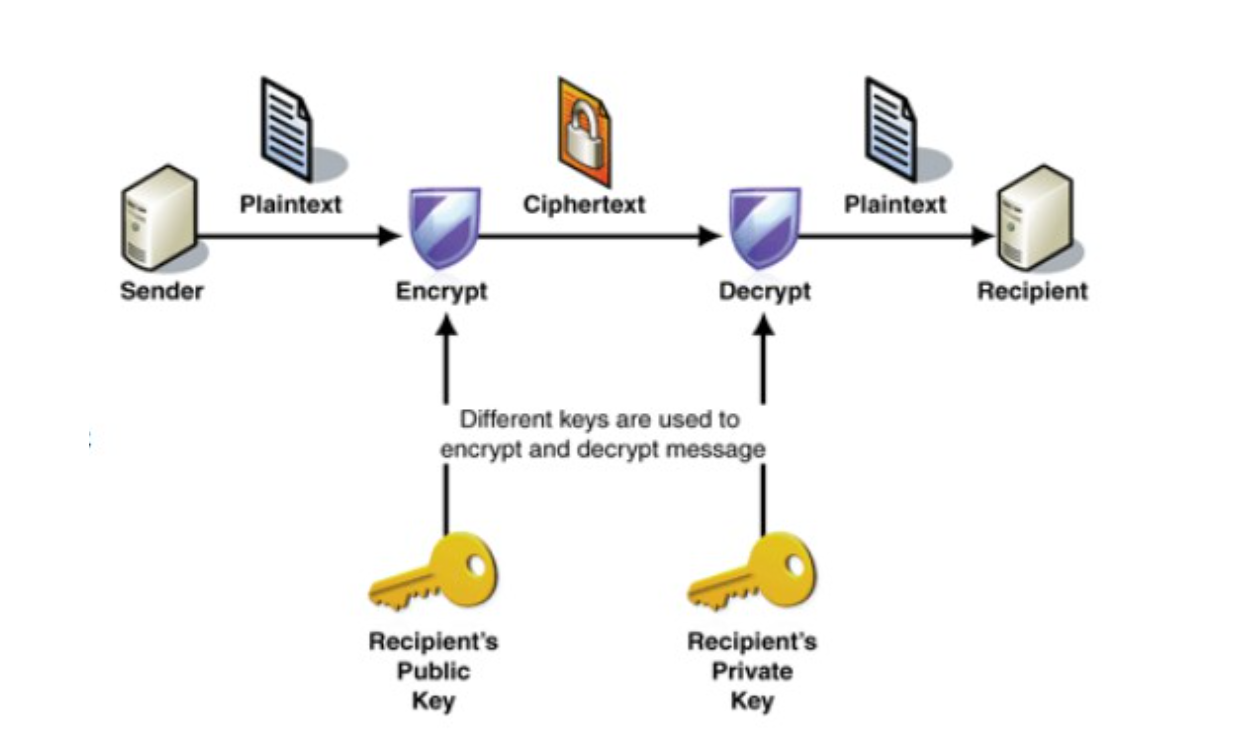
\includegraphics[height=75mm, width=150mm]{pubblica}
Una importante propriet\'a di questo algoritmo \'e:
\begin{verbatim}
Kd( Ke (Messaggio)) = Ke( Kd (Messaggio)) = Messaggio
\end{verbatim}
Questo consente di poter applicare le chiave in 2 modi diversi ottenendo 2 diverse funzioni:
\begin{itemize}
\item \textbf{Privacy (crypt/decrypt)}:\\ A deve inviare un messaggio P riservato a B su di un canale insicuro.
B possiede una coppia di chiave asimmetriche Be (privata) e Bd (pubblica).
A cifra P con la chiave pubblica di B: C= Bd(P). Solo B pu\'o decifrarlo P=Be(C)
\item \textbf{Autenticazione e Integrit\'a (sign/verify)}:\\
A deve inviare un messaggio P attraverso un canale insicuro. Tutti lo possono leggere, ma chi lo riceve deve essere sicuro che \'e stato inviato da A.
A possiede una coppia di chiave asimmetriche Ae (privata) e Ad (pubblica).
A cifra P con la propria chiave privata: C= Ae (P). Chiunque pu\'o applicare la chiave pubblica di A: P=Ae(C). La decifratura funziona solo se P \'e stato cifrato da A.
\end{itemize}
\subsection{Implementazione nell'applicazione}
Nella nostra applicazione abbiamo utilizzato l'algoritmo a chiave pubblica per lo scambio di messaggi in modo sicuro.\\
Dopo essersi autenticati con successo la nostra applicazione si occupa della creazione della coppia di chiavi pubblica-privata attraverso la classe \textbf{Encryptor}.
Quando si vuole inviare un messaggio criptato il client chiede al server di recapitargli la chiave pubblica del destinatario. In questo modo il client pu\'o scegliere di cambiare la coppia di chiavi in qualunque momento. L'algoritmo a chiave pubblica utilizzato \'e l'RSA con chiave 1024bit.

\section{Sviluppi futuri}
Si potrebbe dare continuit\'a a questo progetto aggiungendo alcune features:
\begin{itemize}
\item Si potrebbe pensare di implementare l'autenticazione in CAS da noi solo studiata ma non implementata.
\item la nostra applicazione non tiene conto delle amicizie tra utenti.
\end{itemize}
\newpage
\section{Strumenti utilizzati}
Il progetto \'e stato scritto interamente con Eclisse Version: Kepler Service Release 2\\

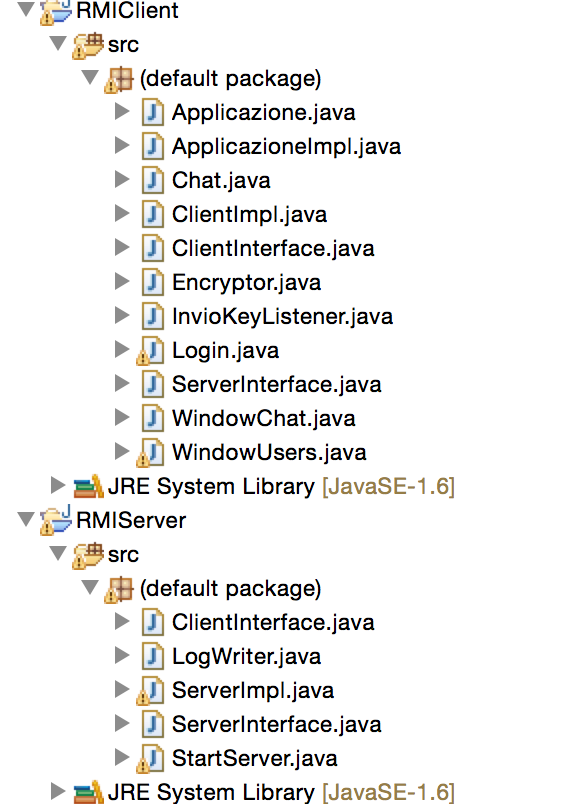
\includegraphics[height=75mm, width=55mm]{img}

La relazione \'e stata scritta in LaTeX
  \end{document}